\documentclass{standalone}

\usepackage{tikz}
\usepackage{ctex}

\begin{document}
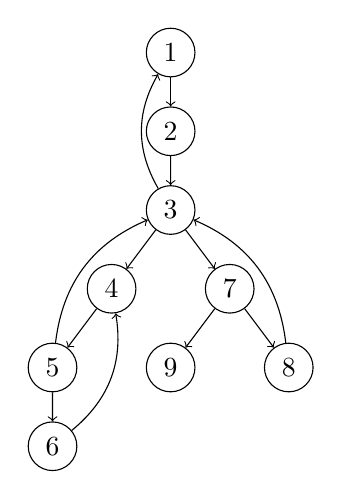
\begin{tikzpicture}
    [level distance=1cm,every node/.style={draw,circle}]

\node (A) {$1$}
    child[->] {node (B) {$2$}
        child {node (C) {$3$}
            child {node (D) {$4$}
                child {node (E) {$5$}
                    child {node (F) {$6$}}
                }
                child[missing]
            }
            child {node (G) {$7$}
                child {node (I) {$9$}}
                child {node (H) {$8$}}
            }
        }
    };

\path[->]
    (C) edge[bend left] (A)
    (E) edge[bend left] (C)
    (F) edge[bend right] (D)
    (H) edge[bend right] (C);

\end{tikzpicture}
\end{document}
